%%%%%%%%%%%%%%%%%%%%%%%%%%%%%%%%%%%%%%%%%
% Academic Title Page
% LaTeX Template
% Version 2.0 (17/7/17)
%
% This template was downloaded from:
% http://www.LaTeXTemplates.com
%
% Original author:
% WikiBooks (LaTeX - Title Creation) with modifications by:
% Vel (vel@latextemplates.com)
%
% License:
% CC BY-NC-SA 3.0 (http://creativecommons.org/licenses/by-nc-sa/3.0/)
% 
% Instructions for using this template:
% This title page is capable of being compiled as is. This is not useful for 
% including it in another document. To do this, you have two options: 
%
% 1) Copy/paste everything between \begin{document} and \end{document} 
% starting at \begin{titlepage} and paste this into another LaTeX file where you 
% want your title page.
% OR
% 2) Remove everything outside the \begin{titlepage} and \end{titlepage}, rename
% this file and move it to the same directory as the LaTeX file you wish to add it to. 
% Then add \input{./<new filename>.tex} to your LaTeX file where you want your
% title page.
%
%%%%%%%%%%%%%%%%%%%%%%%%%%%%%%%%%%%%%%%%%

%----------------------------------------------------------------------------------------
%	PACKAGES AND OTHER DOCUMENT CONFIGURATIONS
%----------------------------------------------------------------------------------------

\documentclass[11pt]{article}

\usepackage[utf8]{inputenc} % Required for inputting international characters
\usepackage[T1]{fontenc} % Output font encoding for international characters

\usepackage{mathpazo} % Palatino font
\usepackage{hyperref} % must be loaded before apacite
\hypersetup{
    colorlinks=true,
    linkcolor=blue, % internal
    filecolor=magenta, % unused
    urlcolor=cyan, % external
    citecolor=blue, % internal
}
\usepackage{mdframed} % For placeholder notes
\usepackage{apacite} % Because Mila likes APA
\usepackage{multicol} % For the multicolumn lists
\usepackage{graphicx} % Include graphics
\usepackage{minted} % Add formatted source code

\graphicspath{ {images/} }


\begin{document}

%----------------------------------------------------------------------------------------
%	TITLE PAGE
%----------------------------------------------------------------------------------------

\begin{titlepage} % Suppresses displaying the page number on the title page and the subsequent page counts as page 1
	\newcommand{\HRule}{\rule{\linewidth}{0.5mm}} % Defines a new command for horizontal lines, change thickness here
	
	\center % Centre everything on the page
	
	%------------------------------------------------
	%	Headings
	%------------------------------------------------
	
	\textsc{\LARGE Thompson Rivers University}\\[1.5cm] % Main heading such as the name of your university/college
	
	\textsc{\Large COMP 4610}\\[0.5cm] % Major heading such as course name
	
	\textsc{\large Advanced Databases}\\[0.5cm] % Minor heading such as course title
	
	%------------------------------------------------
	%	Title
	%------------------------------------------------
	
	\HRule\\[0.4cm]
	
	{\huge\bfseries Big Dota Reduction: Analyzing Over One Billion Dota 2 Matches}\\[0.4cm] % Title of your document
	
	\HRule\\[1.5cm]
	
	%------------------------------------------------
	%	Author(s)
	%------------------------------------------------
	
	\begin{minipage}{0.2\textwidth}
		\begin{flushleft}
			\large
			\textit{Author}\\
			Marco \textsc{Lussetti} % Your name
		\end{flushleft}
	\end{minipage}
	~
	\begin{minipage}{0.2\textwidth}
		\begin{flushleft}
			\large
			\textit{Author}\\
			Dyson \textsc{Fraser} % Your name
		\end{flushleft}
	\end{minipage}
	~
	\begin{minipage}{0.2\textwidth}
		\begin{flushright}
			\large
			\textit{Supervisor}\\
			Dr. Mila \textsc{Kwiatkowska} % Supervisor's name
		\end{flushright}
	\end{minipage}
	
	% If you don't want a supervisor, uncomment the two lines below and comment the code above
	%{\large\textit{Author}}\\
	%John \textsc{Smith} % Your name
	
	%------------------------------------------------
	%	Date
	%------------------------------------------------
	
	\vfill\vfill\vfill % Position the date 3/4 down the remaining page
	
	{\large\today} % Move back a day} % Date, change the \today to a set date if you want to be precise
	
	%------------------------------------------------
	%	Logo
	%------------------------------------------------
	
	%\vfill\vfill
	%\includegraphics[width=0.2\textwidth]{placeholder.jpg}\\[1cm] % Include a department/university logo - this will require the graphicx package
	 
	%----------------------------------------------------------------------------------------
	
	\vfill % Push the date up 1/4 of the remaining page
	
\end{titlepage}

%----------------------------------------------------------------------------------------

\addtocounter{page}{1} % Start counting at title page

\begin{mdframed}[linewidth=2pt]

	\emph{List of Responsabilities:} the two co-authors worked jointly on the project and it would not be feasible to assign responsability for most individual sections and tasks due to the overlap of duties.

	\emph{Note \#1:} this report is based on our work as submitted in the course of our previous submissions during the course as well as our submission to the TRU Undergraduate Conference. We have omitted direct citations to the submission outside of this paragraph for convenience purposes and as they form the same body of work \cite{lussettiBigDataReduction2019}.
	
	\emph{Note \#2:} the full source code for this report, as well as for the poster, and the implementation of utilities \& analysis necessary for this project are available on GitHub at \href{https://github.com/marcolussetti/opendotadump-tools}{marcolussetti/opendotadump-tools}. This includes a README pointing to the key files and folders in the repository.
\end{mdframed}

\section{Introduction} % DONE

The availability of large data sets of player choices in popular online computer games presents an opportunity to identify sudden changes in choice patterns and explore what factors may contribute to such changes. This would be a form of time-series analysis, with the seasonality determined at least partially by meta-game events rather than exclusively the Gregorian calendar. It is thought that industry is ahead of academia in working with very large data sets \cite{jinSignificanceChallengesBig2015} and we hope that by showcasing the feasibility of poor man's solutions to very large data sets we can help encourage academics with limited resources to undertake big data work.

We are particularly interested in exploring one of the largest publicly available data sets, a data set from the OpenDota Project \cite{theopendotaprojectFAQ2014} containing all matches played in the online video game Dota 2 over five years due to its large size and detail \cite{theopendotaprojectDataDumpMarch2017}. We are interested in analyzing the big data reduction techniques required to handle such data sets, as well as the engineering challenges involved in processing a data set that cannot be stored in memory in its initial form and thus must be handled via stream processing. Of great interest to us are approaches and techniques that are viable with the limited computing resources that may be available to individual researches or small teams.

\subsection{What is Dota 2?} % DONE

Dota 2 is a online multiplayer game that has two teams of 5 players each competing to destroy each others Ancient, a large structure located in the center of their base. To win the game one team's ancient must be destroyed but there are many obstacles that stop teams from rushing in and destroying it in the opening minutes of a match. There is a large jungle separating the two bases with three paths, or lanes as they are more commonly called, leading from one base to the other. The half of the lane is part of one team's territory and the other half belongs to the other team. Turrets are stationed on each teams half in order to hinder progress to the Ancient.

Players choose from a list of playable characters call Heroes at the start of each match and level them up by killing creeps (Non Playable Characters spawned from the Ancient), other non-playing characters that are located in the jungle and enemy heroes. The experience points that players gain by playing a Hero does not transfer to another match. Heroes have been designed for a specific role that causes them to mainly be played in one of these lanes. For example there is a type of character called a Carry that is very frail but can do lots of damage, this type of character in combination with a Support(another role) play together in the same lane. Hero picks are a very important part of the game and I would now like to explain the mechanics behind hero selection. At the start of each game, players pick from the pool of heroes, 115 heroes exist but at the time our data was collected only 111 were released, once one player on a team has picked a hero no other player on that team can pick that hero for that match. The result after picking heroes is a unique set of characters that must be leveled up over the course of the match. Players often migrate to a specific role such as carry or support and only play characters within that select role as that is what is most enjoyable for them. So their Hero pick pool is shrunk from 111 to ~30. Within this group of ~30 heroes players must now decided who to play and there are many things to take into account when choosing a Hero most importantly is how good that character is.

The state of viability for a hero varies as time passes. If a hero is picked too much or their win ratio is too high Valve, the developers of Dota 2, will update the game and implement changes that will make the hero worse. This is known as a Nerf, an update to a over powered item or character in a game that takes away some of its power in order to balance the other items and characters of the game. Inversely, if a character or item is under powered a Buff can take place which makes the item or character better in hopes of raising its win ratio or pick rate to similar levels as its contemporaries. Nerfs and buffs are both implemented in the game in the form of updates more commonly known as Patches. Based on the current power level of a Hero, it may become a more desirable pick among players. Another thing that may sway a player's choice would be the implementation of a new Hero that fulfills a role that the player enjoys to play. These new heroes are also introduced via patches.

\subsection{Research Objectives} % DONE

\begin{itemize}
    \item Detect metagame shifts from hero pick ratios, that would be caused by external events (patches to the game, major tournaments, etc.)
    \item “Tame” the dataset’s enormity using the simplest tools possible, and using only the resource of a normal machine as may be available to an average researcher without extensive funding
\end{itemize}

\section{Methodology} % DONE

\subsection{Materials} % DONE

Our research relied on the Open Dota Data Dump, a data dump published by the Open Dota project in 2017. This is a collection of meta data on 1.2 billion matches over five years \cite{theopendotaprojectDataDumpMarch2017}. It consists of three files extracted from the same collection of meta data. \emph{match\_skill} provides information on the Valve-estimated skill level of the match, \emph{matches} provides meta data about all matches in the data set, and \emph{player\_matches} provides detailed in-match data about a subset of matches. Our research will use the \emph{matches} file as we are only interested in basic meta data about each match, and were interested in having as matches to work on as possible. It should be noted that while sample files exist for all these files, the \emph{player\_matches} file is no longer accessible from its original torrent due to lack of seeders.

The \emph{matches} file is a comma-separated value file with 27 columns, one of which, $pgroup$ is an embedded JSON fields. Figure \ref{fig:matchesFile} shows the attributes of this file. The asterisk denotes the columns we have identified as possibly needed for our analysis.

\begin{figure}[h]
  \centering
    \caption{Fields in $matches$ file}
    \label{fig:matchesFile}
    \begin{mdframed}[linewidth=2pt]
        \begin{multicols}{2}
            \begin{itemize}
                \item $match\_id$
                \item $match\_seq\_num$
                \item $radiant\_win ^{*}$
                \item $start\_time ^{*}$
                \item $duration$
                \item $tower\_status\_radiant$
                \item $tower\_status\_dire$
                \item $barracks\_status\_radiant$
                \item $barracks\_status\_dire$
                \item $cluster$
                \item $first\_blood\_time$
                \item $lobby\_type$
                \item $human\_players$
                \item $leagueid$
                \item $positive\_votes$
                \item $negative\_votes$
                \item $game\_mode$
                \item $engine$
                \item $picks\_bans$
                \item $parse\_status$
                \item $chat$
                \item $objectives$
                \item $radiant\_gold\_adv$
                \item $radiant\_xp\_adv$
                \item $teamfights$
                \item $version$
                \item $pgroup ^{*}$
            \end{itemize}
        \end{multicols}
    \end{mdframed}
\end{figure}

\subsection{Methods} % DONE

\subsubsection{Big Data Reduction In Theory}
Because of the large size of the data set, we quickly determined that we would need to not only employ dimensionality reduction to reduce its size before analyzing, but to also aggregate it at some level.

The issues associated with high dimensionality data sets are well understood, and in our context chiefly relate to the increased storage requirement and computational complexity required to handle such data set. In our case, the sparsity issues that might be associated with high dimensionality are not a real concern for our study because of the large size of the data set itself and the fact that we are not using the data set to make prediction relying on these dimensions \cite{poreMustKnowWhatCurse2017, urrehmanBigDataReduction2016}. In terms of dimensionality reduction thus, we were able to condense our data set to merely the heroes picked, the time of the match, and which team won.

However, dimensionality reduction alone would not condense the data set significantly enough to allow for processing on our limited resources. We established this by manually creating a dimensionality reduced-version of 637309 lines, the average lines per day. While this benchmark is admittedly crude as all lines are identical, it did give us some idea of what we could achieve via dimensionality reduction alone. One day represented in this manner amounted to 94.8 MB, which compared to the original dimension of 670.56 MB ($1.12TB/1870 days$) represented a compression of approximately 7 times. Thus the complete data set would be estimated at around 160GB, a significant reduction but alas not enough.

Our next step in condensing the data is to examine whether any viable option exists for granularity reduction. The concept of an information granule is used in granular computing to indicate the minimum unit employed in the model. Thus, the larger the granule can be thought of as being, the more information it abstracts away \cite{yaoGranularComputing2004}. In our case, we are attempting to compare days rather than individual matches, and thus can aggregate hero picks on a day by day basis. We can think of our information granule as moving from being an individual match to being a day of matches treated as an individual unit. In our benchmarking, again using repeated entries, we estimated that decreasing the granularity of the data would yield a 2.73 KB per day file which would be an approximately 34600 times reduction.

\subsubsection{Big Data Reduction Implementation} % DONE

We implemented both dimensionality and granularity reduction jointly as a Java utility. We chose Java as a performant language with a large selection of libraries.

We need to keep in mind that the data set cannot be loaded into memory at once and thus must be treated as a form of stream. However, we do have the advantage of the stream being bounded, and thus may do without a real-time stream processing stream. Stream processing is well understood and is normally tackled by solutions such as cloud computing \cite{iyerWhatDrivesBig2013} or tools like Hadoop or Spark \cite{namiotBigDataStream2015}. However, because we intended to avoid deploying significant computing resources as would be needed to set up a cluster, we developed our own \emph{poor man's solution} to process the data set.

We originally intended to and experimented with using Java 8 Streams to avoid having to decompress the match data set and adopt a more modern interface, however we quickly determined that the streams introduced significant overhead and were not well suited for the size of data we needed to process.

The input file we are seeking to process is a comma separated value file. We originally investigated the feasibility of developing our own barebone parser, however that it was not a viable option due to the complexity involved. We investigated several options for Java CSV parsing libraries. General purpose CSV parsing libraries like $opencsv$ \cite{ruckerjonesOpencsv2019} do not possess adequate performance (in our early trials we saw performance as low as 1,000 records per second). We reviewed benchmarks for CSV libraries that suggested that the fastest library may be univocity-Parsers \cite{univocitysoftwareptyltdComparisonsAllJavabased2018}. However when we attempted to implement a univocity-Parser \cite{univocitysoftwareptyltdUniVocityparsers2019} based-solution in our utility, we discovered that while the performance claims may well be justified, the library did not cope well with large amounts of records. We found that it would use as much as 16GB of RAM to process only 400,000 records and increasing the allocation of memory to the JVM to 24 GB only allowed an additional 50,000 records to be processed. We thus decided to investigate alternative libraries that might have a thinner memory footprint. We settled on the second fastest library in the benchmark, SimpleFlatMapper \cite{rogerSimpleFlatMapper2019}. This library allowed us very good performance (peaking at 100,000 records per second) while maintaining a low memory footprint. We treated all columns as strings, and only performed parsing on the necessary columns.

The $pgroup$ field is an embedded JSON field so we chose to rely on Jsoniter \cite{wenJsoniterJsoniterator2019} as a JSON parser. The library's performance appeared adequate so we did not investigated the matter significantly. We liked that it did not strongly bound to classes unlike some other libraries thus allowing for faster prototyping.

We also investigated more memory-efficient data structures for holding the resulting data, for which we relied on Trove4J \cite{edenGNUTroveTrove4j2013} library which produces some interesting memory efficiency gains for HashMaps \cite{vorontsovTroveLibraryUsing2014}. However, this proved to be a premature optimization that was wholly unnecessary due to the small size of the HashMaps used in the program.

Last we should note that we relied on picocli \cite{popmaPicocli2019} for the command line interface implementation.

The Java implementation of this portion is available as \nameref{subsec:matches-condenser} or on our GitHub repository as the \\\href{https://github.com/marcolussetti/opendotadump-tools/tree/master/matches_condenser}{matches\_condenser} utility.

Some additional conversion tools in the pipeline are implemented in Python and available as \nameref{subsec:json-to-csv} or in our GitHub repository as the \href{https://github.com/marcolussetti/opendotadump-tools/tree/master/json_to_csv}{json\_to\_csv} tool which includes parts of the needed data cleansing and processing.

\subsubsection{Extraction of Metagame Shifts} % DONE

To detect the shifts in the metagame, we decided to attempt a very low tech approach. One may imagine each day as a vector of 111 dimensions where each dimension represents the pick rate for a given hero (thus all of those pick rates always add up to 1). We decided to compare each day's vector to a vector representing the running average of the last two weeks (14 days). We used Manhattan distance to compare the vectors.

This produces a comparable value over time, where we may identify prominent peaks as highlighting changes in the metagame. This is well suited to visual identification: the peaks are slowly absorbed over time as they are incorporated into the running average thus creating a peak both in height and width (representing respectively the level of change and the time taken for the new changes to become the normal metagame).

This was implemented as a set of Jupyter Notebook, which also produced the graphs used in this document and the previous presentation. They may be reviewed as \nameref{subsec:lookup-spikes} or in our GitHub repository under our \href{https://github.com/marcolussetti/opendotadump-tools/tree/master/analysis/heroes_picks}{analysis} tools.

\section{Results}

In first place, we were able to produce an aggregate chart of the pick ratios, which shows the pick ratios of all champions over time. This is visible in Figure \ref{fig:pick-ratios-stacked-all}, however it is impossible to reproduce the chart with adequate details in this context and we recommend reviewing the full scale chart in its entirety which is referred to in the chart's caption.

\begin{figure}
    \centering
    \caption{All Heroes Pick Ratios \href{https://raw.githubusercontent.com/marcolussetti/opendotadump-tools/master/poster/plots/poster_stacked_white_44x12.png}{(full size)}}
    \label{fig:pick-ratios-stacked-all}
    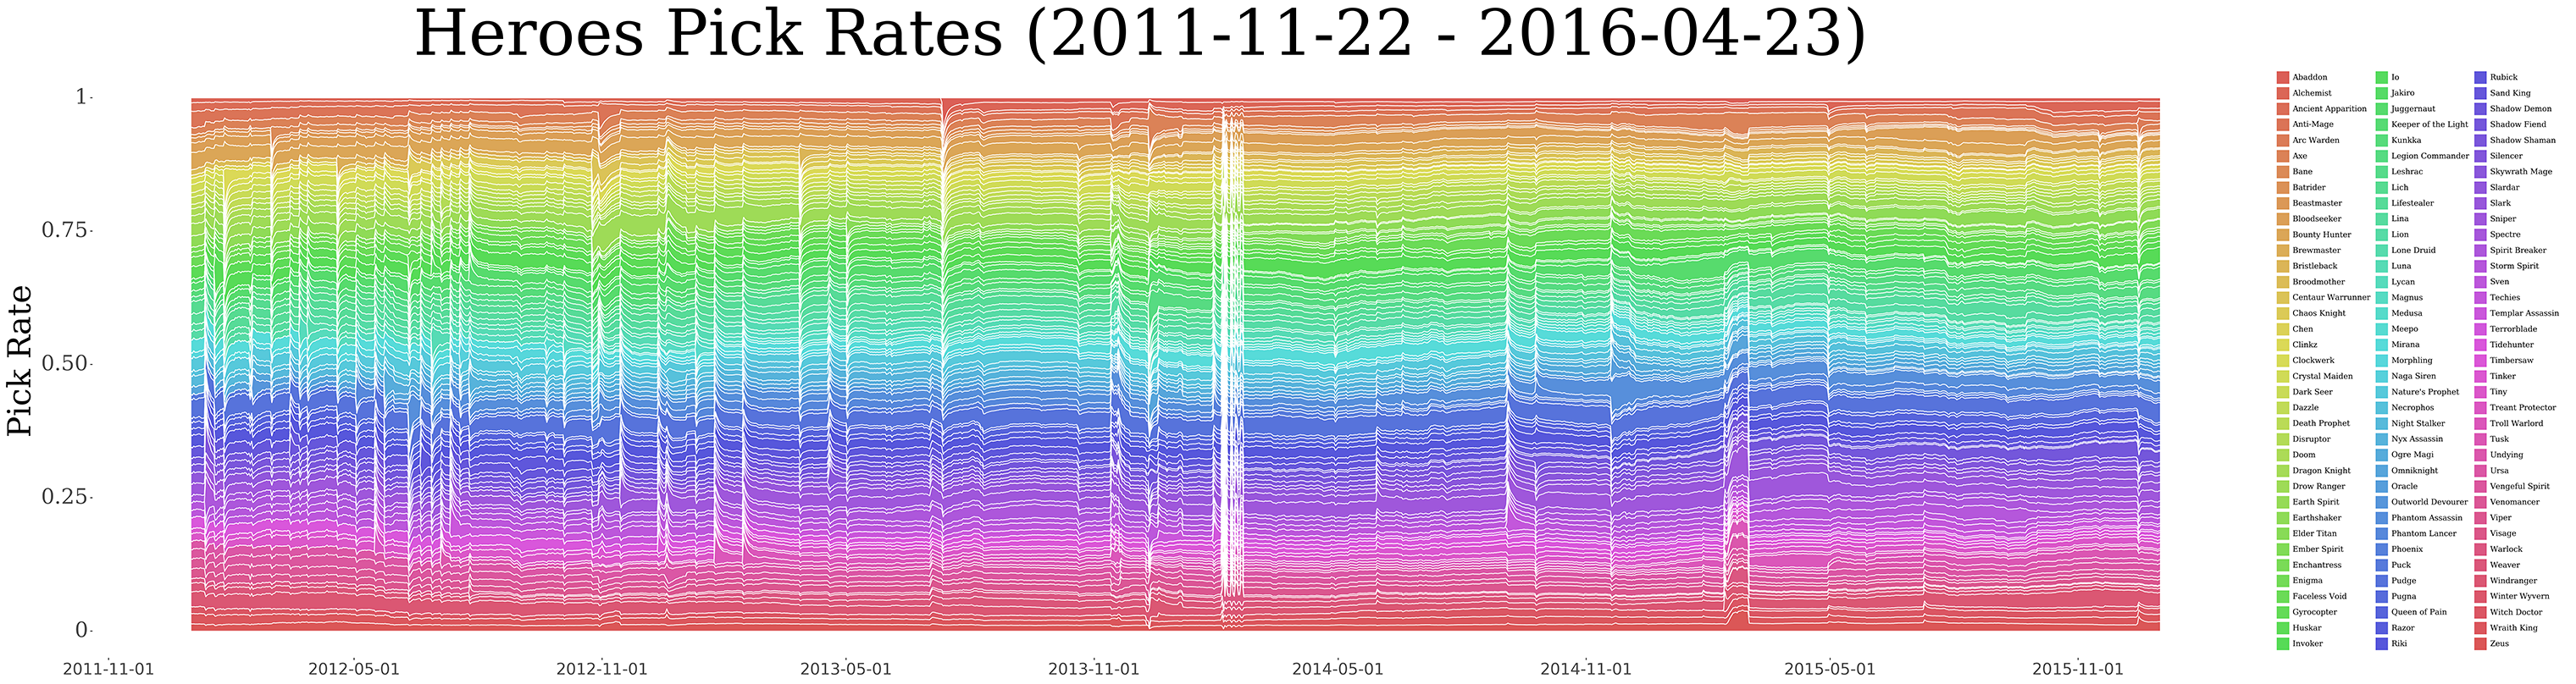
\includegraphics[angle=90,origin=c,height=0.6\textheight]{poster_stacked_white_44x12_025_3041x808.png}
\end{figure}

From our analysis of the Manhattan distance of each day to the running average of the last two weeks, we were able to produce a representation of metagame change points which may be seen in Figure \ref{fig:pick-ratios-differences-labelled-all}. We have manually highlighted some of the more prominent peaks which we will attempt to identify the causing event for. This can be seen in Figure \ref{fig:patches-list}.

\begin{figure}[p]
    \centering
    \caption{All Heroes Difference \href{https://raw.githubusercontent.com/marcolussetti/opendotadump-tools/master/poster/differences_labelled.png}{(full size)}}
    \label{fig:pick-ratios-differences-labelled-all}
    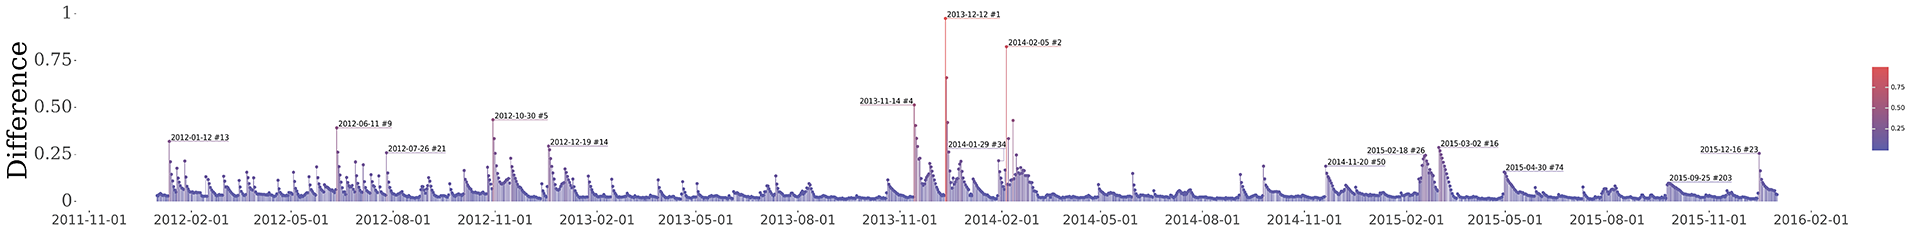
\includegraphics[angle=90,origin=c,height=0.5\textheight]{differences_labelled_1920x231.png}
\end{figure}

\begin{figure}[p]
    \centering
    \caption{List of major metagame shifts}
    \label{fig:patches-list}
    \begin{mdframed}[linewidth=2pt]
        \begin{itemize}
            \item \emph{2012-01-12} Major rebalancing of heroes \& item changes (\nameref{fig:20120112})
            \item \emph{2012-06-11} Chaos Knight, Phantom Assassin, Gyrocopter released (\nameref{fig:20120611})
            \item \emph{2012-07-26} Nyx Assassin, Keeper of the Light, Visage released (\nameref{fig:20120726})
            \item \emph{2012-10-30} Recently released Centaur Warrunner is nerfed (\nameref{fig:20121030})
            \item \emph{2012-12-19} Major rebalance of most/all champions (\nameref{fig:20121219})
            \item \emph{2013-11-14} Three Spirits Patch, significant out-of-game \& economy changes (\nameref{fig:20131114})
            \item \emph{2013-12-12} Skeleton King removed shortly before, Legion Commander added, Wraith King added shortly after (\nameref{fig:20131212})
            \item \emph{2014-01-29} Terrorblade, Phoenix released (\nameref{fig:20140119})
            \item \emph{2014-02-05} Year Beast Brawl (special game mode) (\nameref{fig:20140205})
            \item \emph{2014-11-20} Oracle released (\nameref{fig:20141120})
            \item \emph{2015-02-18} Year Beast Brawl (special game mode) (\nameref{fig:20150218})
            \item \emph{2015-04-30} Major balance changes (\nameref{fig:20150430})
            \item \emph{2015-05-03} No major changes, but The Summit 3 Tournament tickets released (\nameref{fig:20150503})
            \item \emph{2015-09-25} Major balance changes (prev. day) (\nameref{fig:20150925})
            \item \emph{2015-12-16} Arc Warden released (\nameref{fig:20151216})
        \end{itemize}
    \end{mdframed}
\end{figure}

As may be seen in the figures, we believe our algorithm was successful in identifying major metagame shifts. Most major peaks could be tracked down to specific patches issued by the developer, and we did not see sizable shifts caused by tournaments such as The International. We did run our analysis with other options such as median instead of average of the pick rates, 28 days average rather than 14 days, and other distance measures such as euclidian distance. We did not see significant enough differences to warrant further investigation at this stage.

We produced some additional material such as the pick rate for the most popular heroes (see figure \ref{fig:pick-ratios-top-10-popular-all}) and for the heroes with the highest variability (see figure \ref{fig:pick-ratios-top-10-variation}).

\begin{figure}[h]
    \centering
    \caption{Top 10 Heroes by Pick Rate Average \href{https://raw.githubusercontent.com/marcolussetti/opendotadump-tools/master/prints/picks_most_popular/printout_most_popular_point_15x4_5.png}{(full size)}}
    \label{fig:pick-ratios-top-10-popular-all}
    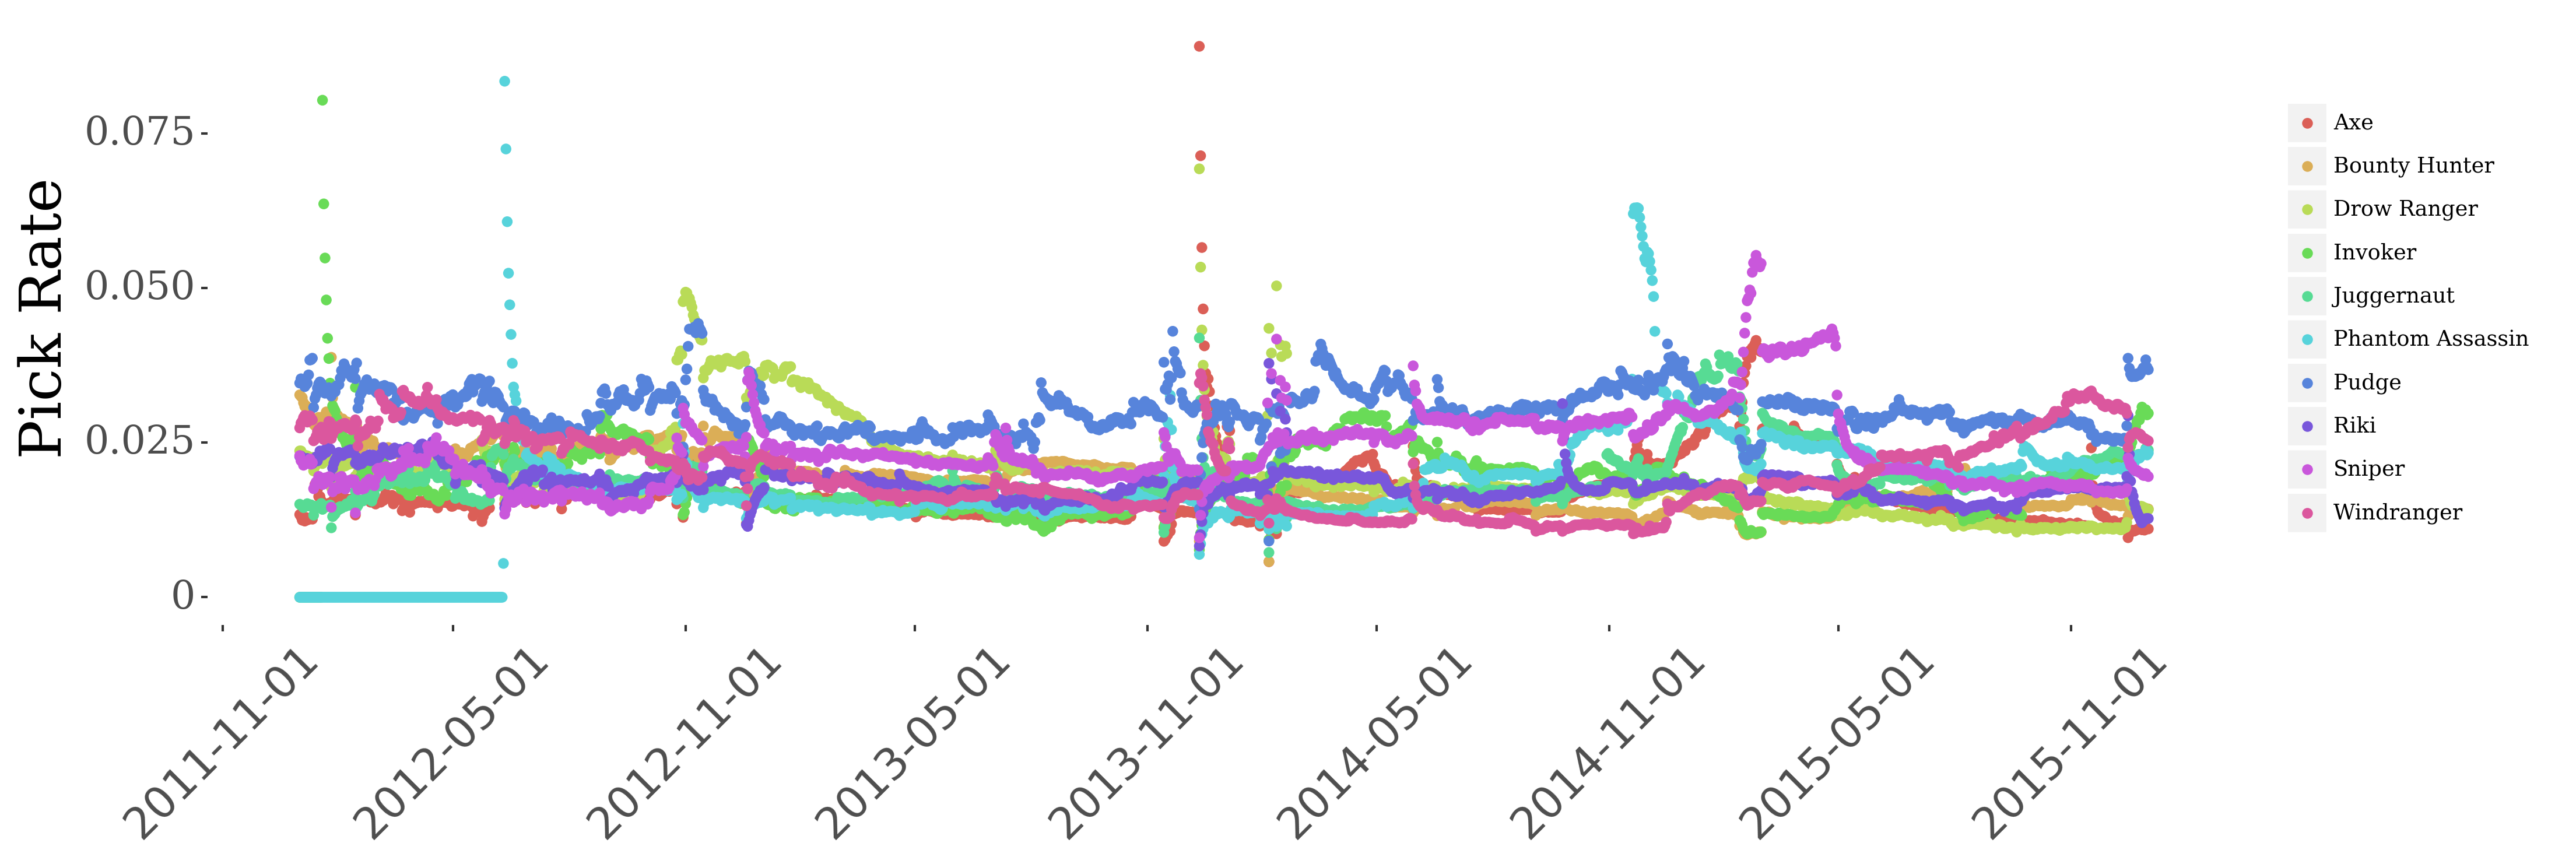
\includegraphics[width=1\textwidth]{printout_most_popular_point_15x4_5.png}
\end{figure}

\begin{figure}[h]
    \centering
    \caption{Top 10 Heroes by Variation (Std. Dev.) \href{https://raw.githubusercontent.com/marcolussetti/opendotadump-tools/master/prints/picks_highest_variability_heroes/printout_most_variation_point_15x4_5.png}{(full size)}}
    \label{fig:pick-ratios-top-10-variation}
    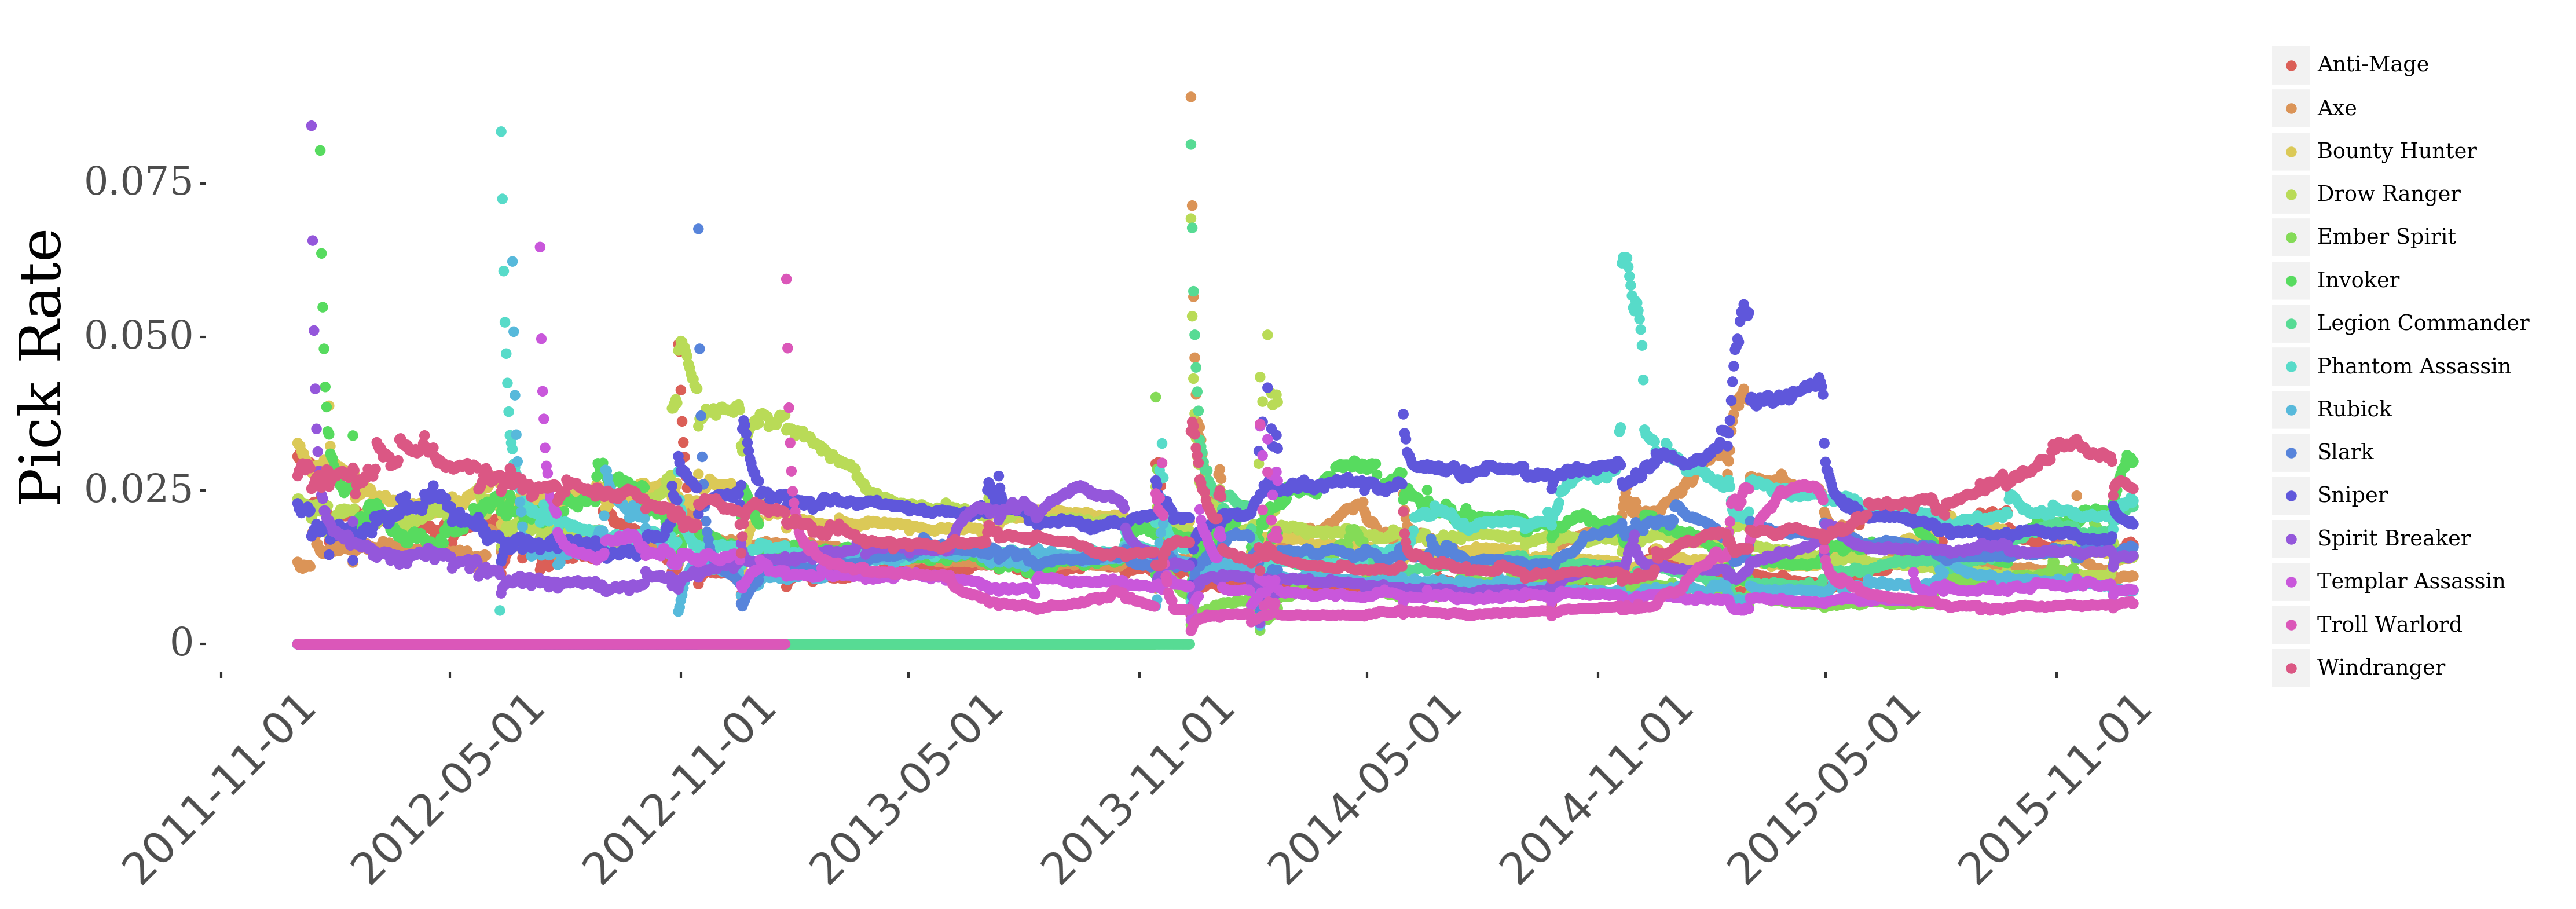
\includegraphics[width=1\textwidth]{printout_most_variation_point_15x4_5.png}
\end{figure}

\section{Discussion}

We have identified a number of shortcomings and good areas for future work.

\emph{Game Types}. Currently all game modes were treated as one, but this includes game modes where players are playing versus the AI, random heroes modes, and various draft modes where picks and bans are used to choose heroes. This was largely acceptable for our initial results, but we were advised that this was responsible for some of the most significant spikes which related to the limited time release of unique game modes. As such, while we are correctly detecting major metagame events, it might be beneficial to normalize away such unique game modes and focus only on the major, more traditional, game modes to produce more balance-oriented metrics.

\emph{Win Ratios}. We have started to look at wins and losses for each heroes. This has the potential to provide us with greater insights on trends in the metagame as it would not only allow us to evaluate how often a hero is chosen, but also how successful that hero is in actual gameplay. This might be a better indicator of underlaying changes in the game rather than changes in popularity. The divergence between these two metrics could provide insight as to the inflexibility of some heroes' popularity. We have produced some preliminary results that indicate that win ratio might be far more nuanced than pick rate. For instance, we can see that examining the win ratios of the top 10 most popular heroes (see figure \ref{fig:winratio-top10-differences}) will yield very similar characteristics to the overall winratio differences chart (see figure \ref{fig:winratio-differences}), whereas doing so for just the pick rate of the top 10 most popular champion does not do so.

\begin{figure}[H]
    \centering
    \caption{Difference for Top 10 Most Popular Heroes, Win Ratio \href{https://raw.githubusercontent.com/marcolussetti/opendotadump-tools/master/prints/winratios_differences/poster_winratio_differences_top_10_15x4_5.png}{(full size)}}
    \label{fig:winratio-top10-differences}
    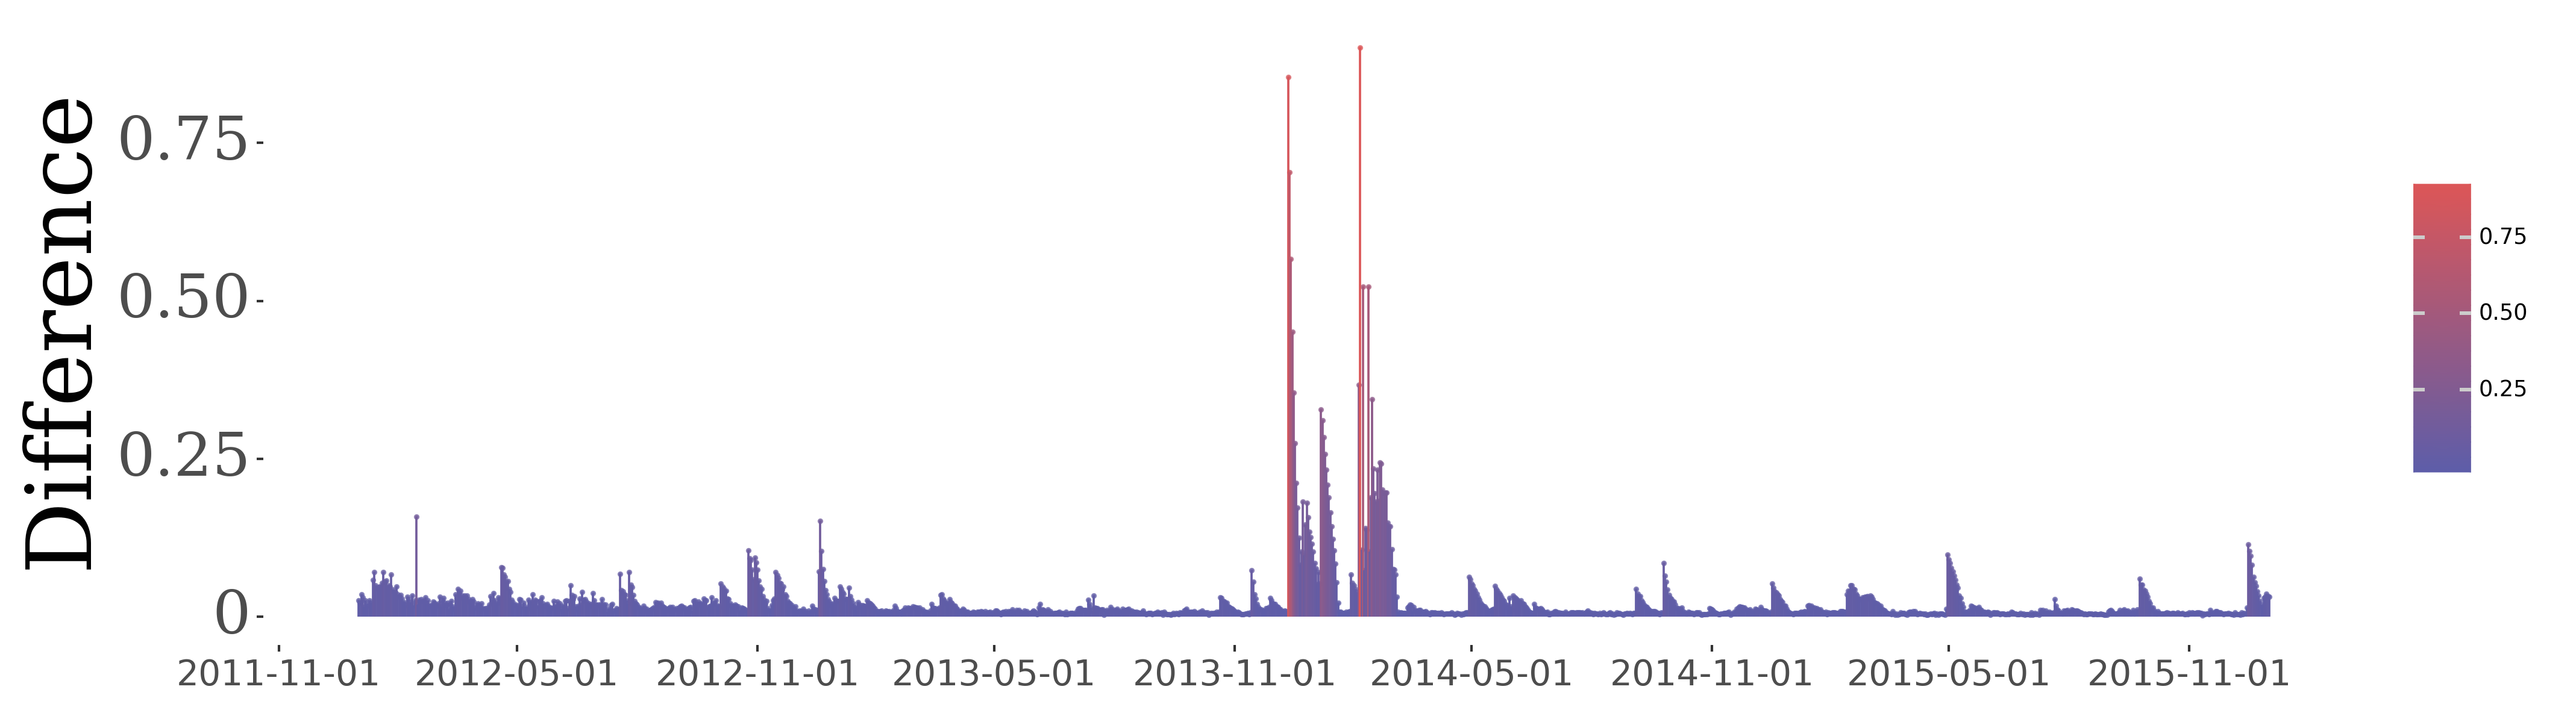
\includegraphics[width=1\textwidth]{poster_winratio_differences_top_10_15x4_5_small.png}
\end{figure}

\begin{figure}[H]
    \centering
    \caption{Difference for All Heroes, Win Ratio \href{https://raw.githubusercontent.com/marcolussetti/opendotadump-tools/master/prints/winratios_differences/poster_winratio_differences_white_15x4.5.png}{(full size)}}
    \label{fig:winratio-differences}
    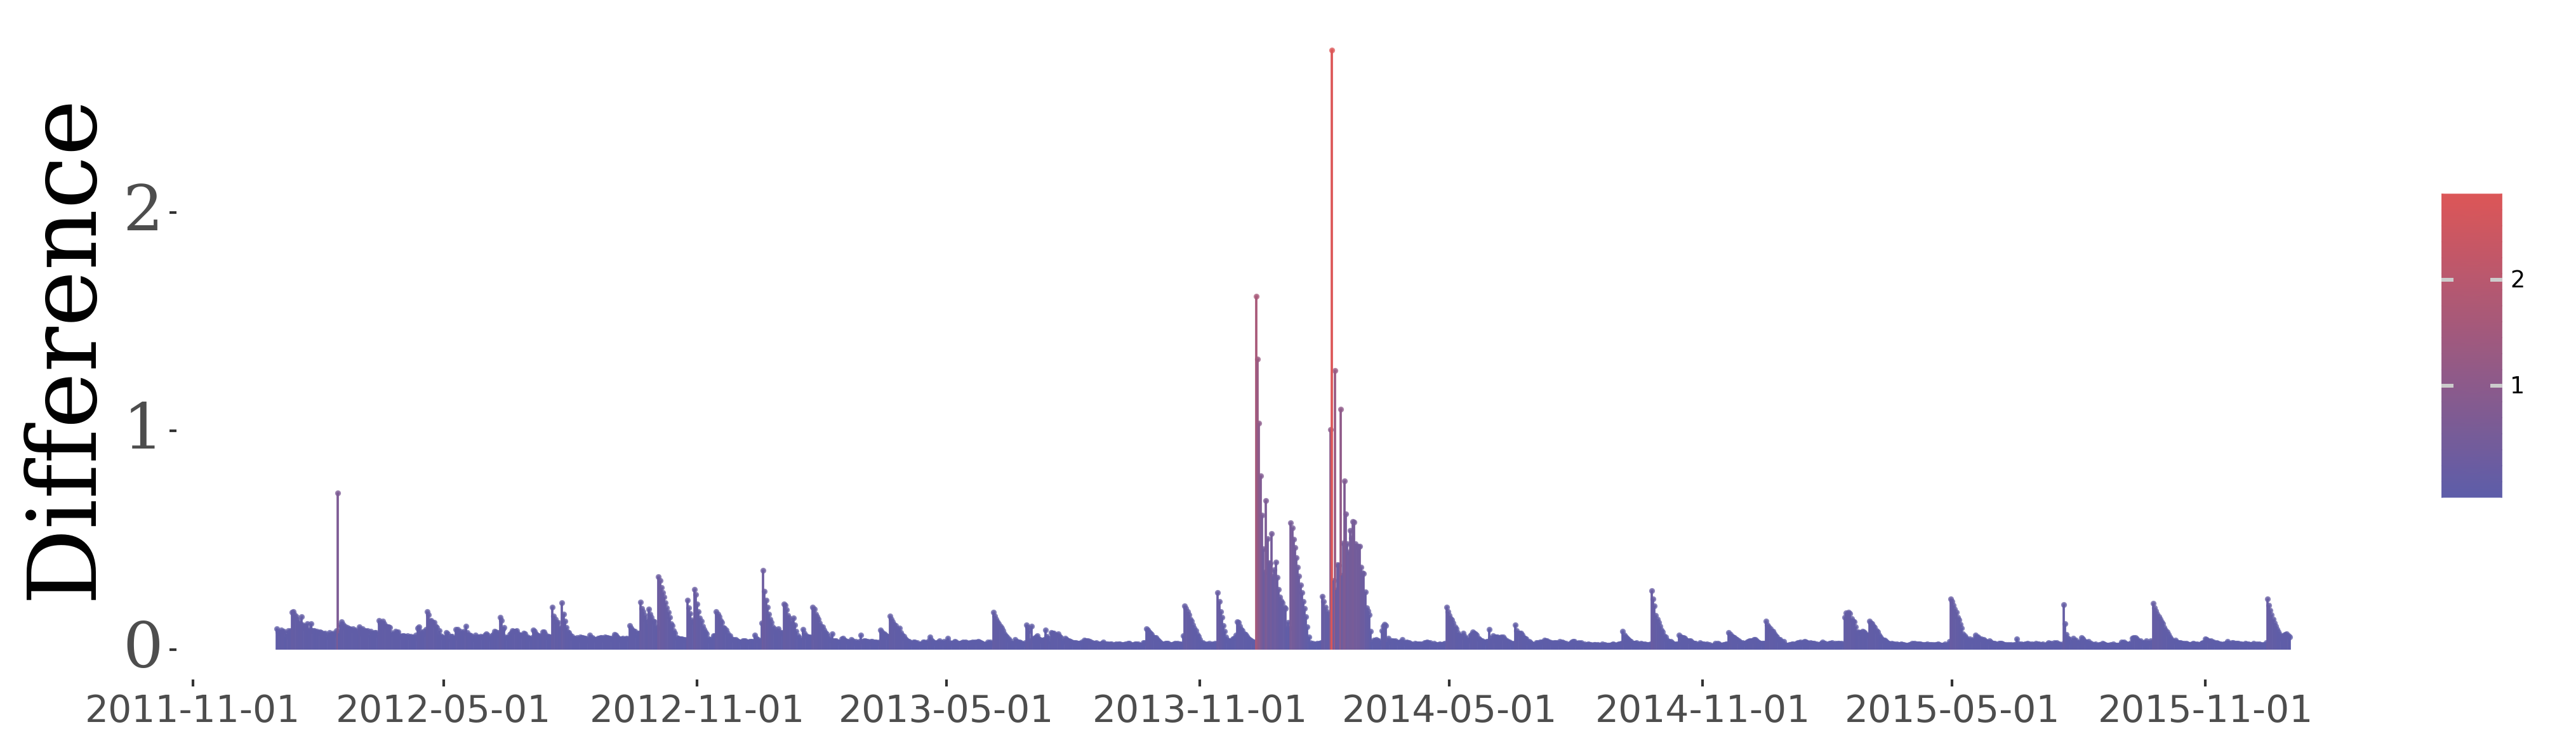
\includegraphics[width=1\textwidth]{poster_winratio_differences_white_15x45_small.png}
\end{figure}

\emph{Skill Levels}. We suspect players of different skill levels might react with different timeframes or different intensity to metagame changes. For instance, we detected no overly significant changes connected to tournaments but wonder whether players of a higher skill level might react to such subtler signals. We could avail ourselves of the $matches\_skill$ file and/or infer the skill level from the game mode played to explore these sort of results.

\emph{Increased Granularity}. We would like to reprocess the data for a hourly-granularity rather than daily to be able to explore reaction times to patches in more detail.

\emph{Interactive Visualization}. We have found it challenging to explore our static visualization because of their high dimensionality, and suspect that we might be able to produce a much clearer visualization if we used interactive technologies such as D3.js that would allow for selectively choose the data points to visualize.

\emph{Roles}. As we noted in the Introduction, Dota 2 fill different \& specific roles. We would like to investigate whether we could cluster the heroes or perform some correlation analysis to discover the roles from the underlaying data such as heroes that are picked together, heroes that are picked in response to other heroes, and so on. We could compare this data with data provided by subject matter experts as to what they perceive the roles to be, or lists available online from that timeperiod.

\section{Three Questions} % DONE

\subsection{What is the Curse of Dimensionality?}

"[E]xponential growth in data causes high sparsity in the data set and unnecessarily increases storage space and processing time" \cite{poreMustKnowWhatCurse2017}

\subsection{Can you explain the difference between Granularity reduction and Dimensionality reduction?}
Dimensionality reduction trims the number of attributes recorded (=less columns) whereas to reduce granularity is to reduce the level of detail at which the data is recorded (= less rows).

\subsection{What does the size of a granule in represent in granular computing?}
The (inverse) degree of abstraction of your model. The larger your granules are, the higher the abstraction in your model. \cite{yaoGranularComputing2004}

\bibliographystyle{apacite}
\bibliography{Report}

\section*{Appendixes} % DONE

\subsection*{\emph{Appendix A:} matches\_condenser -> Main.java}
\label{subsec:matches-condenser}

\href{https://github.com/marcolussetti/opendotadump-tools/blob/master/matches_condenser/src/main/java/com/marcolussetti/opendotamatchescondenser/Main.java}{See on GitHub}

\begin{minted}[linenos,breaklines]{java}
package com.marcolussetti.opendotamatchescondenser;

import com.jsoniter.JsonIterator;
import com.jsoniter.any.Any;
import com.jsoniter.output.JsonStream;
import gnu.trove.map.hash.THashMap;
import gnu.trove.set.hash.THashSet;
import org.simpleflatmapper.csv.CsvParser;
import picocli.CommandLine;
import picocli.CommandLine.Option;
import picocli.CommandLine.Command;
import picocli.CommandLine.Parameters;

import java.io.*;
import java.time.*;
import java.time.format.DateTimeFormatter;
import java.util.*;
import java.util.concurrent.Callable;
import java.util.concurrent.TimeUnit;

@Command(description = "Process OpenDota Matches File",
        name = "processopendota",
        mixinStandardHelpOptions = true,
        version = "processopendota 0.3")
class ProcessOpenDota implements Callable<Void> {
    // ARGUMENTS
    @Option(names = {"-x", "--extract-to-json"},
            description = "Extract an existing .ser file to a JSON file.")
    private File extractToJson = null;

    @Option(names = {"-c", "--condense"},
            description = "Condense the input openDota CSV file. If file is GunZipped (.gz), extract it first.")
    private File condense = null;

    @Option(names = {"-o", "--only-count"},
            description = "Only count picks, do not record wins & losses")
    private Boolean onlyCount = false;

    @Parameters(paramLabel = "OUTPUT",
            description = "Output file for either extract or condense")
    private File output = null;

    // CONSTANTS
    public static final int MATCHES_NO = 1191768403;
    public static final int DAYS_NO = 1870;
    public static final int REPORT_THRESHOLD = 1000000; // Report progress every million rows
    public static final int SERIALIZE_THRESHOLD = 10000000; // Serialize every 10 million rows

    // VARIABLES
    // Keep track of progress
    private LocalDateTime startOfParsing;
    private THashSet<Long> allDates = new THashSet<>();
    private int recordCounter = 0;
    // Store the data {date: Long, {hero#: int -> picks# int}}
    private THashMap<Long, THashMap<Integer, Integer[]>> data = new THashMap<>();

    private void condenseInputFile(File input, File output, boolean onlyCount) {
        this.startOfParsing = LocalDateTime.now();

        // Main loop!
        FileReader fileReader;
        try {
            fileReader = new FileReader(input);
            Iterator<String[]> csvReader = CsvParser.iterator(fileReader);
            String[] headers = csvReader.next();
            // Iterate through stuff
            while (csvReader.hasNext()) {
                String[] row = csvReader.next();

                parseRow(row, onlyCount);

                if (recordCounter % REPORT_THRESHOLD == 0) {
                    reportProgress(this.recordCounter, this.allDates.size(), this.startOfParsing);

                    if (recordCounter % SERIALIZE_THRESHOLD == 0) {
                        String destFolder = output.getParent();
                        String[] destFile = output.getName().split("\\.");
                        File outputFile = new File(destFolder + File.separator + destFile[0] + "_" + (recordCounter / SERIALIZE_THRESHOLD) + "." + destFile[1]);

                        serializeData(data, outputFile);
                    }
                }
            }

            reportProgress(this.recordCounter, this.allDates.size(), this.startOfParsing);
            serializeData(data, output);
        } catch (IOException e) {
            e.printStackTrace();
        }

    }

    private void extractToJson(File input, File output) {
        THashMap<Long, THashMap<Integer, Integer[]>> hashMap = deserializeData(input);

        writeJSON(hashMap, output);
    }

    private void parseRow(String[] row, boolean onlyCount) {
        // Extract relevant fields
        long startTime = Long.parseLong(row[3]);
        String pgroup = row[26];
        boolean radiantWin = row[2].equals("t");

        // Parse date
        Long date = extractDate(startTime).toEpochDay();

        // Parse picks
        ArrayList<Integer[]> heroesPicked = extractHeroesPicked(pgroup, radiantWin);

        // Update copy of local map
        THashMap<Integer, Integer[]> todayPicks = this.data.getOrDefault(date, new THashMap<Integer, Integer[]>());
        heroesPicked.forEach(heroRecord -> {
            int hero = heroRecord[0];
            boolean won = heroRecord[1] == 1;

            Integer[] counts = todayPicks.getOrDefault(hero, new Integer[]{0, 0});
            if (onlyCount || won)
                counts[0] += 1;
            else
                counts[1] += 1;
            todayPicks.put(hero, counts);
        });

        // Push to global map
        this.data.put(date, todayPicks);

        // Tracking progress
        allDates.add(date);
        recordCounter++;
    }

    private static LocalDate extractDate(long epochTimeInSeconds) {
        return LocalDateTime.ofInstant(
                Instant.ofEpochSecond(epochTimeInSeconds),
                ZoneId.of("UTC")
        ).toLocalDate();
    }

    private static ArrayList<Integer[]> extractHeroesPicked(String jsonInput, boolean radiantWon) {
        ArrayList<Integer[]> heroes = new ArrayList<>();

        JsonIterator iterator = JsonIterator.parse(jsonInput);
        Map<String, Any> jsonObject = null;
        try {
            jsonObject = iterator.read(Any.class).asMap();
        } catch (IOException e) {
            e.printStackTrace();
        }

        jsonObject.forEach((index, object) -> {
            int heroId = object.get("hero_id").toInt();
            boolean isRadiant = object.get("player_slot").toInt() <= 127;
            Integer[] heroRecord = {heroId, ((isRadiant && radiantWon) || (!isRadiant && !radiantWon)) ? 1 : 0 };
            heroes.add(heroRecord);
        });

        return heroes;

    }

    private static void reportProgress(int recordCounter, int days, LocalDateTime startOfParsing) {
        Duration elapsed = Duration.between(startOfParsing, LocalDateTime.now());
        long elapsedMillis = elapsed.toMillis();
        DateTimeFormatter dtf = DateTimeFormatter.ofPattern("yyyy/MM/dd HH:mm:ss");
        double rowsPerSec = (double) recordCounter / elapsedMillis * 1000;

        System.out.printf(
                "\n%s (%s elapsed - %s remaining) | %9.2f rows/s | %,6.2f million rows (%6.2f%%)| %4d days (%6.2f%%)",
                dtf.format(LocalDateTime.now()),                                                // current time
                formatTimeDifference(elapsedMillis),                                            // elapsed time
                formatTimeDifference((long) ((MATCHES_NO - recordCounter) / rowsPerSec * 1000)),// remaining time (est.)
                (double) recordCounter / elapsedMillis * 1000,                                  // rows per second
                (double) recordCounter / 1000000,                                               // rows processed (mils)
                (double) recordCounter / MATCHES_NO * 100,                                      // % of rows processed
                days,                                                                           // days tracked
                days / (float) DAYS_NO * 100                                                    // % of days tracked
        );
    }

    private static String formatTimeDifference(long millis) {
        // From https://stackoverflow.com/a/44142896/6238740
        return String.format(
            "%02d:%02d:%02d",
            TimeUnit.MILLISECONDS.toHours(millis),
            TimeUnit.MILLISECONDS.toMinutes(millis) - TimeUnit.HOURS.toMinutes(
                TimeUnit.MILLISECONDS.toHours(millis)
            ),
            TimeUnit.MILLISECONDS.toSeconds(millis) - TimeUnit.MINUTES.toSeconds(
                TimeUnit.MILLISECONDS.toMinutes(millis)
            )
        );
    }

    private static void serializeData(THashMap<Long, THashMap<Integer, Integer[]>> data, File output) {

        // From https://beginnersbook.com/2013/12/how-to-serialize-hashmap-in-java/
        FileOutputStream fos = null;
        try {
            fos = new FileOutputStream(output);
            ObjectOutputStream oos = new ObjectOutputStream(fos);
            oos.writeObject(data);
            oos.close();
            fos.close();
        } catch (IOException e) {
            e.printStackTrace();
        }
        System.out.print("\n> Saved data to " + output.getAbsolutePath());
    }

    public static THashMap<Long, THashMap<Integer, Integer[]>> deserializeData(File file) {
        // From https://beginnersbook.com/2013/12/how-to-serialize-hashmap-in-java/
        THashMap<Long, THashMap<Integer, Integer[]>> hashMap;
        try {
            FileInputStream fis = new FileInputStream(file);
            ObjectInputStream ois = new ObjectInputStream(fis);
            hashMap = (THashMap<Long, THashMap<Integer, Integer[]>>) ois.readObject();
            ois.close();
            fis.close();
        } catch (IOException ioe) {
            ioe.printStackTrace();
            return null;
        } catch (ClassNotFoundException c) {
            System.out.println("Class not found");
            c.printStackTrace();
            return null;
        }
        return hashMap;
    }

    public static void writeJSON(THashMap<Long, THashMap<Integer, Integer[]>> hashMap, File outputFile) {

        String output = JsonStream.serialize(hashMap);
        try {
            outputFile.createNewFile();
        } catch (IOException e) {
            e.printStackTrace();
        }

        try (PrintStream out = new PrintStream(new FileOutputStream(outputFile))) {
            out.print(output);
            out.flush();
        } catch (FileNotFoundException e) {
            e.printStackTrace();
        }

    }

    public static void main(String[] args) {
        CommandLine.call(new ProcessOpenDota(), args);
    }

    @Override
    public Void call() throws Exception {
        // BUSINESS LOGIC

        if (extractToJson == null && condense == null) {
            System.out.println("Well you need to select something... try --help");
            return null;
        }
        if (extractToJson != null && condense != null) {
            System.out.println("Can't have it both ways... try --help");
            return null;
        }
        if (output == null) {
            System.out.println("Must provide an output file!");
            return null;
        }

        if (extractToJson != null) {
            System.out.println("Converting from SER to JSON");
            extractToJson(extractToJson, output);
            System.out.println("Conversion complete: " + output.getAbsolutePath());
        }
        if (condense != null) {
            System.out.println("Condensing from CSV to SER");
            condenseInputFile(condense, output, onlyCount);
            System.out.println("Condensing complete: " + output.getAbsolutePath());
        }

        return null;
    }
}
\end{minted}

\subsection*{\emph{Appendix B:} json\_to\_csv -> opendota\_jsontocsv.py}
\label{subsec:json-to-csv}

\href{https://github.com/marcolussetti/opendotadump-tools/blob/master/json_to_csv/opendota_jsontocsv.py}{See on GitHub}

\begin{minted}[linenos,breaklines]{python}
#!/usr/bin/env python3
"""OPENDOTA_JSONTOCSV

Usage:
    opendota_jsontocsv.py JSON_INPUT_FILE CSV_OUTPUT_FILE [--heroes=(names|numbers)] [(-n | --normalize)] [(-r | --remove-low-counts)]
    opendota_jsontocsv.py JSON_INPUT_FILE CSV_OUTPUT_FILE --picks-by-hero [--remove-low-counts] [--heroes=(names|numbers)] [(-r | --remove-low-counts)]
    opendota_jsontocsv.py JSON_INPUT_FILE CSV_OUTPUT_FILE --picks-by-date [--remove-low-counts] [(-r | --remove-low-counts)]
    opendota_jsontocsv.py (-h | --help)
    opendota_jsontocsv.py --version

Options:
    -h --help                   Show this screen.
    --version                   Show version.
    --heroes=(names|numbers)    Record heroes by name or number [default: names].
    -n --normalize              Normalize picks as proportion of picks per day.
    -r --remove-low-counts         Removes early records (pre 2011-11-22) as they have lower volumes of recorded matches.
    --picks-by-date             Export the number of picks for each day to CSV.
    --picks-by-hero             Export the number of picks for each hero to CSV.
"""
import datetime

import requests
import pandas as pd
from docopt import docopt


if __name__ == '__main__':
    arguments = docopt(__doc__, version='OpenDotaDumpTools JsonToCsv 0.2')

    print("Starting OpenDotaDumpTools...")

    df = pd.read_json(arguments["JSON_INPUT_FILE"])
    print("JSON input loaded")

    # Clean up data
    df = df.transpose()  # Rotate so rows = time
    df = df.fillna(0)  # Replace missing values with 0
    df = df.drop(0, 0)  # Remove entries with missing date (1970)
    df = df.drop(0, 1)  # Remove entries with a missing hero (0)
    df.index = [datetime.datetime(1970, 1, 1, 0, 0) + datetime.timedelta(index - 1)
                for index in df.index]  # Convert index (epoch days) to time
    df = df.reindex(sorted(df.columns), axis=1)  # Order columns by hero #, ascending
    df = df.sort_index(axis=0)  # Order rows by date, ascending
    for column in df.columns:  # Convert all values from float to integer
        df[column] = df[column].astype('int64')
    print("Input cleaned")

    if arguments["--remove-low-counts"]:
        df = df.loc[df.index > '2011-11-22 00:00:00']
        print("Data for days previous to 2011-11-23 removed")

    # EXPORT
    if arguments["--picks-by-date"]:
        picks_by_day = df.sum(axis=1)
        picks_by_day.to_csv(arguments["CSV_OUTPUT_FILE"])
        print("Exported picks by date data to {}".format(arguments["CSV_OUTPUT_FILE"]))
        exit(0)  # DONE!

    if arguments["--heroes"] == "names":
        # Fetch heroes from OpenDota API
        heroes_json = requests.get("http://api.opendota.com/api/heroes/").json()
        heroes = {hero["id"]: hero for hero in heroes_json}
        df.columns = [heroes[column]["localized_name"] for column in df.columns]
        print("Heroes ids replaced with heroes names")

    # EXPORT
    if arguments["--picks-by-hero"]:
        picks_by_day = df.sum(axis=0)
        picks_by_day.to_csv(arguments["CSV_OUTPUT_FILE"])
        print("Exported picks by hero data to {}".format(arguments["CSV_OUTPUT_FILE"]))
        exit(0)  # DONE!

    if arguments["--normalize"]:
        df = df.div(df.sum(axis=1), axis=0)
        print("Values normalized")

    # EXPORT
    df.to_csv(arguments["CSV_OUTPUT_FILE"])
    print("Exported data to {}".format(arguments["CSV_OUTPUT_FILE"]))
\end{minted}

\clearpage

\subsection*{\emph{Appendix C:} Explanatory Tables}
\label{subsec:explanatory-tables}

\begin{figure}[H]
    \centering
    \caption{Explanatory table for 2012-01-12}
    \label{fig:20120112}
    
\includegraphics[width=1\textwidth]{20120112.png}
\end{figure}

\begin{figure}[H]
    \centering
    \caption{Explanatory table for 2012-06-11}
    \label{fig:20120611}
    
\includegraphics[width=1\textwidth]{20120611.png}
\end{figure}

\begin{figure}[H]
    \centering
    \caption{Explanatory table for 2012-07-26}
    \label{fig:20120726}
    
\includegraphics[width=1\textwidth]{20120726.png}
\end{figure}

\begin{figure}[H]
    \centering
    \caption{Explanatory table for 2012-10-30}
    \label{fig:20121030}
    
\includegraphics[width=1\textwidth]{20121030.png}
\end{figure}

\begin{figure}[H]
    \centering
    \caption{Explanatory table for 2012-12-19}
    \label{fig:20121219}
    
\includegraphics[width=1\textwidth]{20121219.png}
\end{figure}

\begin{figure}[H]
    \centering
    \caption{Explanatory table for 2013-11-14}
    \label{fig:20131114}
    
\includegraphics[width=1\textwidth]{20131114.png}
\end{figure}

\begin{figure}[H]
    \centering
    \caption{Explanatory table for 2013-12-12}
    \label{fig:20131212}
    
\includegraphics[width=1\textwidth]{20131212.png}
\end{figure}

\begin{figure}[H]
    \centering
    \caption{Explanatory table for 2014-01-19}
    \label{fig:20140119}
    
\includegraphics[width=1\textwidth]{20140119.png}
\end{figure}

\begin{figure}[H]
    \centering
    \caption{Explanatory table for 2014-02-05}
    \label{fig:20140205}
    
\includegraphics[width=1\textwidth]{20140205.png}
\end{figure}

\begin{figure}[H]
    \centering
    \caption{Explanatory table for 2014-11-20}
    \label{fig:20141120}
    
\includegraphics[width=1\textwidth]{20141120.png}
\end{figure}

\begin{figure}[H]
    \centering
    \caption{Explanatory table for 2015-02-18}
    \label{fig:20150218}
    
\includegraphics[width=1\textwidth]{20150218.png}
\end{figure}

\begin{figure}[H]
    \centering
    \caption{Explanatory table for 2015-04-30}
    \label{fig:20150430}
    
\includegraphics[width=1\textwidth]{20150430.png}
\end{figure}

\begin{figure}[H]
    \centering
    \caption{Explanatory table for 2015-05-03}
    \label{fig:20150503}
    
\includegraphics[width=1\textwidth]{20150503.png}
\end{figure}

\begin{figure}[H]
    \centering
    \caption{Explanatory table for 2015-09-25}
    \label{fig:20150925}
    
\includegraphics[width=1\textwidth]{20150925.png}
\end{figure}

\begin{figure}[H]
    \centering
    \caption{Explanatory table for 2015-12-16}
    \label{fig:20151216}
    
\includegraphics[width=1\textwidth]{20151216.png}
\end{figure}

\clearpage

\subsection*{\emph{Appendix D:} analysis -> LookupSpikes.ipynb}
\label{subsec:lookup-spikes}

\href{https://github.com/marcolussetti/opendotadump-tools/blob/master/analysis/heroes_picks/LookupSpikes.ipynb}{See on GitHub} - \href{https://colab.research.google.com/github/marcolussetti/opendotadump-tools/blob/master/analysis/heroes_picks/LookupSpikes.ipynb}{Run in Google Colab}

\subsubsection*{Processing}

\emph{Imports \& Configuration}

\begin{minted}[linenos,breaklines]{python}
# Update pandas, just in case
!pip install pandas -U

# If plotnine is not installed:
!pip install plotnine

# If using on google colab, might need to update statsmodels version
!pip install statsmodels -U

# If not installed
!pip install requests
\end{minted}

\emph{Constants for configuration}

\begin{minted}[linenos,breaklines]{python}
CSV_INPUT_FILE = ("https://raw.githubusercontent.com/marcolussetti" "/processopendota/master/data/heroes_picks_csvs/" "stable-picks_heroes-names_normalized.csv")
OPENDOTA_API_HEROES_ENDPOINT = "https://api.opendota.com/api/heroes/"

import pandas as pd
import requests
from plotnine import *
from scipy.spatial import distance
from datetime import datetime, timedelta

%matplotlib inline
\end{minted}

\emph{Import Data}
\begin{minted}[linenos,breaklines]{python}
# Load input csv
df = pd.read_csv(CSV_INPUT_FILE, index_col=0)
\end{minted}

\emph{Examine the data - Overall heroes metrics}
\begin{minted}[linenos,breaklines]{python}
# Most popular heroes overall (mean)
heroes_most_popular = df.mean().sort_values(ascending=False)[:10]  # Average of normalized pick frequency

# Heroes with the most variation
heroes_most_variation = df.std().sort_values(ascending=False)[:15]  # Standard deviation of pick frequency

# Heroes with the least variation
heroes_least_variation = df.std().sort_values(ascending=False)[:10]  # Standard deviation of pick frequency
\end{minted}

\emph{Examine the data - Reformat the data for easy graphing}
\begin{minted}[linenos,breaklines]{python}
df_expl_graph = df.copy(deep=True)
# Condense values
df_expl_graph = df_expl_graph.stack()
df_expl_graph = df_expl_graph.reset_index()

df_expl_graph.columns = ["Day", "Hero", "Frequency"]

df_expl_graph["Day"] = df_expl_graph["Day"].apply(pd.to_datetime)

df_expl_graph["Week"] = df_expl_graph["Day"].apply(lambda date: "{}-{}".format(date.year,date.week))
df_expl_graph["Month"] = df_expl_graph["Day"].apply(lambda date: "{}-{}".format(date.year,date.month))
df_expl_graph["Year"] = df_expl_graph["Day"].apply(lambda date: date.year)

df_most_popular_graph = df_expl_graph[df_expl_graph["Hero"].isin(heroes_most_popular.keys())]
df_most_variation_graph = df_expl_graph[df_expl_graph["Hero"].isin(heroes_most_variation.keys())]
\end{minted}

\emph{Examine the data - Graphs}
\begin{minted}[linenos,breaklines]{python}
all_day_plot = (ggplot(df_expl_graph, aes(x="Day", y="Frequency", color="Hero", group=1))
              +geom_point()
             )
# all_day_plot
# all_day_plot.save("all_day_plot.png", width=40, height=32, dpi=300, limitsize=False)

all_day_stacked_plot = (ggplot(df_expl_graph, aes(x="Day", y="Frequency"))
              +geom_area(aes(fill="Hero"))
             )
# all_day_stacked_plot
# all_day_stacked_plot.save("all_day_stacked_plot.png", width=44, height=12, dpi=300, limitsize=False)
\end{minted}

\emph{Examine the data - Detect changes over time}
\begin{minted}[linenos,breaklines]{python}
def previous_distribution_vector(df, date_start, date_end, average_function="mean"):
  df_filtered = df[(df["Day"] >= date_start) & (df["Day"] < date_end)]
  
  if average_function == "median":
    result = df_filtered.groupby(["Hero"]).median()[["Frequency"]]
  else:
    result = df_filtered.groupby(["Hero"]).mean()[["Frequency"]]
  
  return result.to_dict()["Frequency"]

def compute_distance(day, previous_period_average, distance_function=distance.euclidean, weighted=False):
  previous = [value for key, value 
              in sorted(previous_period_average.items(), key=lambda x: x[0])]
  current = [value for key, value 
              in sorted(day.items(), key=lambda x: x[0])]
  assert len(previous) == len(current), "Incorrect length: previous-> {}, current-> {}".format(len(previous), len(current))
  if weighted:
    return distance_function(previous, current, previous)
  else:
    return distance_function(previous, current)
  
def day_difference(df, day, distance_function=distance.euclidean, length=14, average_function="mean", weighted=False):
  # Extract vector for day
  day_picks = {record["Hero"]: record["Frequency"] for record 
               in df[df["Day"] == day][["Hero", "Frequency"]].to_dict('records')
              }
  previous_picks = previous_distribution_vector(df, datetime.strptime(day, '%Y-%m-%d') - timedelta(days=length), day, average_function)
  
  return compute_distance(day_picks, previous_picks, distance_function, weighted)

def all_days_difference(df, distance_function=distance.euclidean, length=14, average_function="mean", weighted=False):
  all_days = [str(d) for d in sorted(set(date.date() for key, date in df["Day"].to_dict().items()))[1:]]
  
  return {day: day_difference(
      df, day, distance_function=distance_function, 
      length=length, average_function="mean") 
   for day in all_days}
\end{minted}

\emph{Graph differences}
\begin{minted}[linenos,breaklines]{python}
# Try to graph differences for top 10 champions by popularity
pop_differences_by_day = all_days_difference(df_most_popular_graph).items()
sorted_pop_differences_by_day = sorted(pop_differences_by_day, key=lambda x: x[1], reverse=True)
df_pop_differences_by_day = pd.DataFrame(pop_differences_by_day)
df_pop_differences_by_day.columns = ["Day", "Difference"]

popular_heroes_differences_plot = (
    ggplot(df_pop_differences_by_day, aes(x="Day", y="Difference", color="Difference"))
    +geom_point()
    +geom_area(aes(fill="Difference"))
)

# popular_heroes_differences_plot
# popular_heroes_differences_plot.save("pop_differences_plot.png", width=44, height=5, dpi=300, limitsize=False)

# Try to graph differences for all heroes

all_differences_by_day = all_days_difference(df_expl_graph).items()
sorted_all_differences_by_day = sorted(all_differences_by_day, key=lambda x: x[1], reverse=True)
df_all_differences_by_day = pd.DataFrame(all_differences_by_day)
df_all_differences_by_day.columns = ["Day", "Difference"]
df_all_differences_by_day.head()

all_heroes_differences_plot = (
    ggplot(df_all_differences_by_day, aes(x="Day", y="Difference", color="Difference"))
    +geom_point()
    +geom_area(aes(fill="Difference"))
)

# all_heroes_differences_plot
# all_heroes_differences_plot.save("all_differences_plot.png", width=44, height=5, dpi=300, limitsize=False)

# What if we weight it?
# Try to graph differences for all heroes

all_differences_by_day_weighted = all_days_difference(df_expl_graph, weighted=True).items()
sorted_all_differences_by_day_weighted = sorted(all_differences_by_day_weighted, key=lambda x: x[1], reverse=True)
df_all_differences_by_day_weighted = pd.DataFrame(all_differences_by_day_weighted)
df_all_differences_by_day_weighted.columns = ["Day", "Difference"]
df_all_differences_by_day_weighted.head()

all_heroes_differences_weighted_plot = (
    ggplot(df_all_differences_by_day_weighted, aes(x="Day", y="Difference", color="Difference"))
    +geom_point()
    +geom_area(aes(fill="Difference"))
)

# all_heroes_differences_weighted_plot
# all_heroes_differences_plot.save("all_differences_weighted_plot.png", width=44, height=5, dpi=300, limitsize=False)

# Try to graph differences for all heroes, 28 days

all_differences_by_day_28 = all_days_difference(df_expl_graph, length=28).items()
sorted_all_differences_by_day_28 = sorted(all_differences_by_day_28, key=lambda x: x[1], reverse=True)
df_all_differences_by_day_28 = pd.DataFrame(all_differences_by_day_28)
df_all_differences_by_day_28.columns = ["Day", "Difference"]
df_all_differences_by_day_28.head()

all_differences_by_day_28_plot = (
    ggplot(df_all_differences_by_day_28, aes(x="Day", y="Difference", color="Difference"))
    +geom_point()
    +geom_area(aes(fill="Difference"))
)

# all_differences_by_day_28_plot
# all_differences_by_day_28_plot.save("all_differences_28_plot.png", width=44, height=5, dpi=300, limitsize=False)

# Try to graph differences for all heroes, manhattan distance

all_differences_by_day_manhattan = all_days_difference(df_expl_graph, distance_function=distance.cityblock).items()
sorted_all_differences_by_day_manhattan = sorted(all_differences_by_day_manhattan, key=lambda x: x[1], reverse=True)
df_all_differences_by_day_manhattan = pd.DataFrame(all_differences_by_day_manhattan)
df_all_differences_by_day_manhattan.columns = ["Day", "Difference"]

all_heroes_differences_manhattan_plot = (
    ggplot(df_all_differences_by_day_manhattan, aes(x="Day", y="Difference", color="Difference"))
    +geom_point()
    +geom_area(aes(fill="Difference"))
)

# all_heroes_differences_manhattan_plot
# all_heroes_differences_manhattan_plot.save("all_differences_manhattan_plot.png", width=44, height=5, dpi=300, limitsize=False)
\end{minted}

\subsubsection*{Poster Graphs}

\emph{Pick rates by hero (stacked) graph}
\begin{minted}[linenos,breaklines]{python}
poster_stacked = (
    ggplot(df_expl_graph, aes(x="Day", y="Frequency"))
    +geom_area(aes(fill="Hero"), color="white")
    +guides(fill=guide_legend(ncol=3, title="Heroes"))
    +scale_x_datetime(date_breaks="6 months", minor_breaks=4, limits=["2012-01-01", "2016-01-01"])
    +ggtitle("Heroes Pick Rates (2011-11-22 - 2016-04-23)")
    +xlab("")
    +ylab("Pick Rate")
    +theme(
        text=element_text(family=['serif']),
        axis_text=element_text(size=24.0),
        #axis_text_x=element_text(ha="right"),
        axis_title_y=element_text(size=36.0),
        axis_title_x=element_text(size=0.0),
        legend_title=element_blank(),
        plot_title=element_text(size=72.0),
        axis_text_x=element_text(size=18.0, family=['Dejavu Sans', 'Dejavu']),#, angle=45),
        panel_background=element_rect(fill="white", colour="white"),
    )
)
# poster_stacked
poster_stacked.save("poster_stacked_white_46x12.png", width=46, height=12, dpi=300, limitsize=False)
\end{minted}

\emph{Differences graph}
\begin{minted}[linenos,breaklines]{python}
poster_differences_plot = (
    ggplot(df_all_differences_by_day_manhattan, aes(x="Day", y="Difference", color="Difference"))
    +geom_point()
    +geom_area(aes(fill="Difference"))
    +scale_color_gradient(low="#5D5DA9", high="#DC5657")
    +scale_fill_gradient(low="#5D5DA9", high="#DC5657")
    +scale_x_datetime(date_breaks="6 months", minor_breaks=4, limits=["2012-01-01", "2016-01-01"])
    +xlab("")
    +theme(
        text=element_text(family=['serif']),
        panel_background=element_rect(fill="white", colour="white"),
        panel_grid=element_blank(),
        axis_text=element_text(size=24.0),
        axis_title_y=element_text(size=36.0),
        axis_title_x=element_text(size=0.0),
        axis_text_x=element_text(size=18.0, family=['Dejavu Sans', 'Dejavu']),
        legend_text=element_text(family=['Dejavu Sans', 'Dejavu']),
        legend_title=element_blank(),
    )
)

# poster_differences_plot
poster_differences_plot.save("poster_differences_white_41x5.png", width=41, height=5, dpi=300, limitsize=False)
\end{minted}

\emph{Differences graph (3mo)}
\begin{minted}[linenos,breaklines]{python}
poster_differences_plot_3mo = (
    ggplot(df_all_differences_by_day_manhattan, aes(x="Day", y="Difference", color="Difference"))
    +geom_point()
    +geom_area(aes(fill="Difference"))
    +scale_color_gradient(low="#5D5DA9", high="#DC5657")
    +scale_fill_gradient(low="#5D5DA9", high="#DC5657")
    +scale_x_datetime(date_breaks="3 months", minor_breaks=4, limits=["2012-01-01", "2016-01-01"])
    +xlab("")
    +theme(
        text=element_text(family=['serif']),
        panel_background=element_rect(fill="white", colour="white"),
        panel_grid=element_blank(),
        axis_text=element_text(size=24.0),
        axis_title_y=element_text(size=36.0),
        axis_title_x=element_text(size=0.0),
        axis_text_x=element_text(size=18.0, family=['Dejavu Sans', 'Dejavu']),
        legend_text=element_text(family=['Dejavu Sans', 'Dejavu']),
        legend_title=element_blank(),
    )
)

poster_differences_plot_3mo.save("poster_differences_white_41x5_3mo.png", width=41, height=5, dpi=300, limitsize=False)
\end{minted}

\subsubsection*{Explore differences}

\begin{minted}[linenos,breaklines]{python}
# Try to graph differences for all heroes, manhattan distance

all_differences_by_day_manhattan = all_days_difference(df_expl_graph, distance_function=distance.cityblock).items()
differences_by_day_manhattan = all_days_difference(df_expl_graph, distance_function=distance.cityblock)
sorted_all_differences_by_day_manhattan = sorted(all_differences_by_day_manhattan, key=lambda x: x[1], reverse=True)
df_all_differences_by_day_manhattan = pd.DataFrame(all_differences_by_day_manhattan)
df_all_differences_by_day_manhattan.columns = ["Day", "Difference"]

top_differences = {record[0]: {"order": i + 1, "value": record[1]} for i, record in list(enumerate(sorted_all_differences_by_day_manhattan))}

all_differences_by_day_manhattan

top_differences["2015-04-30"]

top_differences
\end{minted}

\subsubsection*{Printout Graphs}

\emph{Most Popular}
\begin{minted}[linenos,breaklines]{python}
poster_stacked = (
    ggplot(df_most_popular_graph, aes(x="Day", y="Frequency"))
    +geom_area(aes(fill="Hero"), color="white")
    +guides(fill=guide_legend(ncol=1, title="Heroes"))
    +scale_x_datetime(date_breaks="6 months", minor_breaks=4, limits=["2012-01-01", "2016-01-01"])
    +ggtitle("Top 10 Overall Most Popular Heroes")
    +xlab("")
    +ylab("Pick Rate")
    +theme(
        text=element_text(family=['serif']),
        axis_text=element_text(size=16.0),
        #axis_text_x=element_text(ha="right"),
        axis_title_y=element_text(size=24.0),
        axis_title_x=element_text(size=0.0),
        legend_title=element_blank(),
        plot_title=element_text(size=24.0),
        axis_text_x=element_text(size=18.0, family=['Dejavu Sans', 'Dejavu'], angle=45),
        panel_background=element_rect(fill="white", colour="white"),
    )
)

poster_stacked

# poster_stacked
poster_stacked.save("printout_most_popular_cumulative_15x4_5.png", width=15, height=4.5, dpi=300, limitsize=False)



poster_stacked = (
    ggplot(df_most_popular_graph, aes(x="Day", y="Frequency"))
    +geom_point(aes(color="Hero"))
    +guides(color=guide_legend(ncol=1, title="Heroes"))
    +scale_x_datetime(date_breaks="6 months", minor_breaks=4, limits=["2012-01-01", "2016-01-01"])
    #+ggtitle("Most PopulHeroes Pick Rates (2011-11-22 - 2016-04-23)")
    +xlab("")
    +ylab("Pick Rate")
    +theme(
        text=element_text(family=['serif']),
        axis_text=element_text(size=16.0),
        #axis_text_x=element_text(ha="right"),
        axis_title_y=element_text(size=24.0),
        axis_title_x=element_text(size=0.0),
        legend_title=element_blank(),
        plot_title=element_text(size=24.0),
        axis_text_x=element_text(size=18.0, family=['Dejavu Sans', 'Dejavu'], angle=45),
        panel_background=element_rect(fill="white", colour="white"),
    )
)

poster_stacked

# poster_stacked
poster_stacked.save("printout_most_popular_point_15x4_5.png", width=15, height=4.5, dpi=300, limitsize=False)
\end{minted}

\emph{Most variation}
\begin{minted}[linenos,breaklines]{python}
poster_stacked = (
    ggplot(df_most_variation_graph, aes(x="Day", y="Frequency"))
    +geom_line(aes(color="Hero"))
    +guides(color=guide_legend(ncol=1, title="Heroes"))
    +scale_x_datetime(date_breaks="6 months", minor_breaks=4, limits=["2012-01-01", "2016-01-01"])
    +ggtitle("Heroes With Highest Variability (Std. Dev.)")
    +xlab("")
    +ylab("Pick Rate")
    +theme(
        text=element_text(family=['serif']),
        axis_text=element_text(size=16.0),
        #axis_text_x=element_text(ha="right"),
        axis_title_y=element_text(size=24.0),
        axis_title_x=element_text(size=0.0),
        legend_title=element_blank(),
        plot_title=element_text(size=24.0),
        axis_text_x=element_text(size=18.0, family=['Dejavu Sans', 'Dejavu'], angle=45),
        panel_background=element_rect(fill="white", colour="white"),
    )
)

poster_stacked


# poster_stacked
poster_stacked.save("printout_most_variation_line_15x4_5.png", width=15, height=4.5, dpi=300, limitsize=False)
\end{minted}

\subsubsection*{Printout Tables}

\begin{minted}[linenos,breaklines]{python}
KEY_DATES = [
    "2012-01-12", "2012-06-11", "2012-07-26", 
    "2012-10-30", "2012-12-19", "2013-11-14", 
    "2013-12-12", "2014-01-19", "2014-02-05", 
    "2014-11-20", "2015-02-18", "2015-04-30", 
    "2015-05-03", "2015-09-25", "2015-12-16"
]

heroes = [hero for hero in df_expl_graph["Hero"]]

two_week_averages = {date: previous_distribution_vector(df_expl_graph, datetime.strptime(date, '%Y-%m-%d') - timedelta(days=14), date, average_function="mean") for date in KEY_DATES}

day_average = {date: {row["Hero"]: row["Frequency"] for id, row in df_expl_graph[df_expl_graph["Day"] == date][["Hero", "Frequency"]].iterrows()} for date in KEY_DATES}

day_difference = {date: {hero: abs(frequency - two_week_averages[date][hero]) for hero, frequency in day_average[date].items()} for date in KEY_DATES}

day_difference_top_10 = {date: (sorted(list(differences.items()), key=lambda x: x[1], reverse=True)[:10]) for date, differences in day_difference.items()}

def process_differences(date, differences):
  results = [("Hero", "Portion of day's shift", "Manhattan distance",
              "Pick for day", "Average pick for 14 prev day")]
  
  total_day_difference = dict(all_differences_by_day_manhattan)[date]
#   for hero in heroes:
#     if hero in [hero in differences] or hero in two_week_averages.keys():
#       results.append((
#           hero,
#           differences[hero] / total_day_difference,
#           differences[hero],
#           day_average[date][hero],
#           two_week_averages[date][hero]
#       ))
  
  for hero, difference in differences:
    results.append((
        hero,
        difference / total_day_difference,
        difference,
        day_average[date][hero],
        two_week_averages[date][hero]
    ))
  
  return results
  
top_10_differences_by_day = {day: process_differences(day, differences) for day, differences in day_difference_top_10.items()}

top_10_differences_by_day

# Write to CSV-ish
with open("explain.csv", "w") as f:
  for date, rows in top_10_differences_by_day.items():
    date_row = (date, "Position: {}".format(top_differences[date]["order"]), "Shift: {}".format(dict(all_differences_by_day_manhattan)[date]))
    for date_component in date_row:
      f.write(date_component)
      f.write(",")
    f.write("\n")
    for row in rows:
      for item in row:
        f.write(str(item))
        f.write(",")
      f.write("\n")
\end{minted}

\end{document}
